
\documentclass[a4j,10pt]{jsarticle}
\usepackage{layout,url,resume}
\usepackage[dvipdfmx]{graphicx}
\pagestyle{empty}

\begin{document}
%\layout

\title{タイトル}

% 和文著者名
\author{
    著者その1 \thanks{所属その1}
    \and
    著者その2 \thanks{所属その2}
}

% 和文概要
\begin{abstract}
ここにアブストラクトを書く。
\end{abstract}

\maketitle
\thispagestyle{empty}

\section{はじめに}

引用例\cite{example}を書いてみた.

\section{背景}

\subsection{hoge}
小見出し付きの文章.

\begin{enumerate}
\item 番号付き箇条書き 
\item 番号付き箇条書き
\end{enumerate}

\begin{itemize}
\item 箇条書き
\item 箇条書き
\end{itemize}

%---------------------------------------------

\section{研究目的}

\subsection{hoge}
hogehoge
画像を貼って見た

\begin{figure}[htbp]
    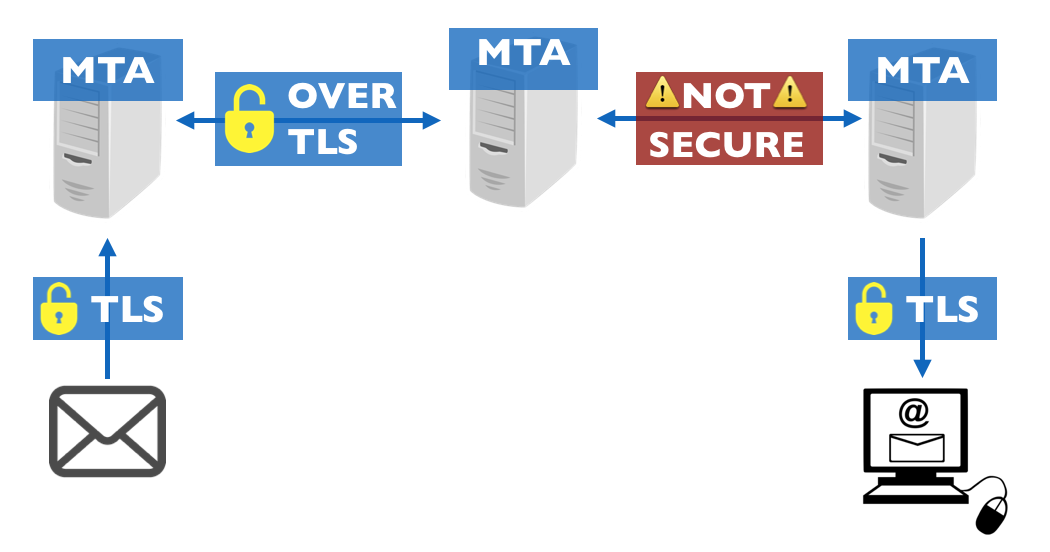
\includegraphics[width=5cm]{figure1.png}
    \caption{}
\end{figure}
 
\subsection{fuga}
fugafuga

\section{関連研究}

\section{提案手法}

\section{評価}

\section{考察}

\begin{thebibliography}{99}
%\bibitem{a}
\bibitem{example}
引用その1\\
\texttt{ http://www.example.com}
\end{thebibliography}

\end{document}
% end of file
